\documentclass[12pt]{article}
% Эта строка — комментарий, она не будет показана в выходном файле
\usepackage{ucs}
\usepackage[warn]{mathtext}
\usepackage[utf8x]{inputenc} % Включаем поддержку UTF8
\usepackage[russian]{babel}  % Включаем пакет для поддержки русского языка
\usepackage{amsmath}
\usepackage{mathtools}
\usepackage{amssymb}
% \usepackage[dvips]{graphicx}
% \graphicspath{{noiseimages/}}
\usepackage[pdftex]{graphicx}


% Параметры страницы: 1см от правого края и 2см от остальных.


\hoffset=0mm
\voffset=0mm
\textwidth=180mm        % ширина текста
\oddsidemargin=-6.5mm   % левое поле 25.4 - 5.4 = 20 мм
\textheight=240mm       % высота текста 297 (A4) - 40
\topmargin=-15.4mm      % верхнее поле (10мм)
\headheight=5mm      % место для колонтитула
\headsep=5mm          % отступ после колонтитула
\footskip=8mm         % отступ до нижнего колонтитула


\begin{document}
    \author {Жарков Андрей 495}
    \title {Лабораторная работа 2.4 \\  Определение вязкости воздуха
    	по скорости течения через тонкие трубки}
    \maketitle{}
    
    \textbf{Цель работы:} экспериментально выявить участки ламинарного и турбулентного течения; определить число Рейнольдса; определить вязкость воздуха; экспериментально определить зависимость расхода воздуха в трубках от радиуса
    
    
    \textbf{В работе используются:} металлические трубки, укрепленные
    на горизонтальной подставке; газовый счетчик; микроманометр
    типа ММН; стеклянная U-образная трубка; секундомер.
    
    \begin{center}
    	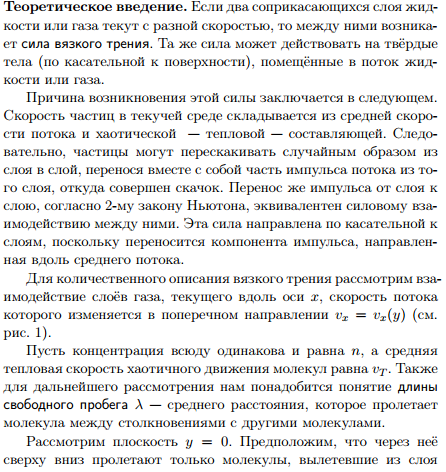
\includegraphics[width=16cm, height=14cm]{theory_0.png}
    	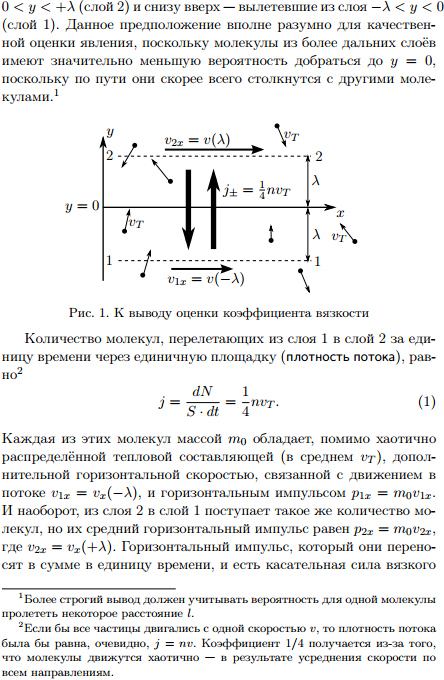
\includegraphics[width=16cm]{theory_1.png}
    	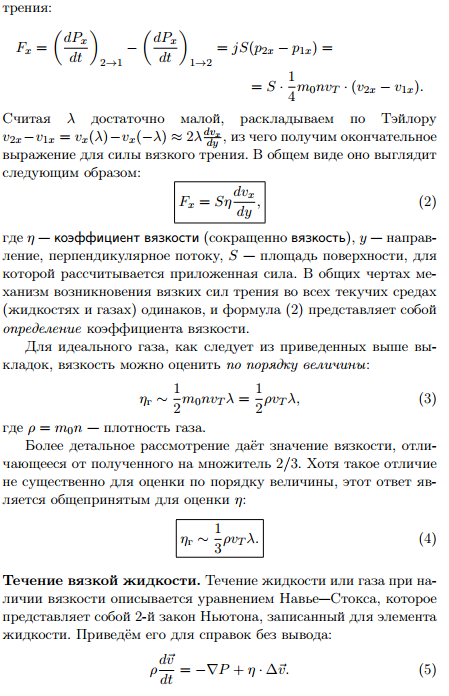
\includegraphics[width=16cm]{theory_2.png}
    	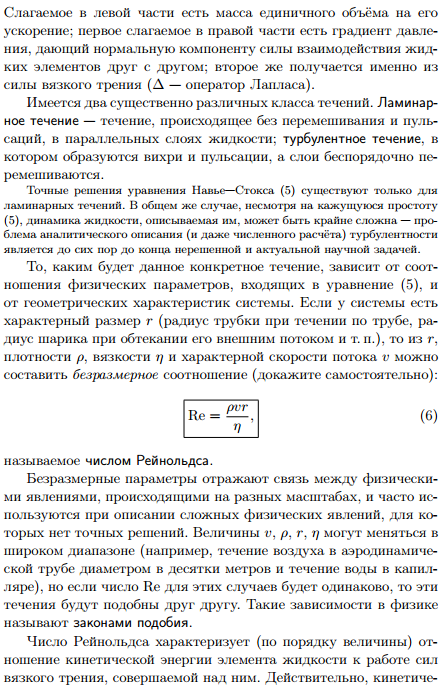
\includegraphics[width=16cm]{theory_3.png}
    	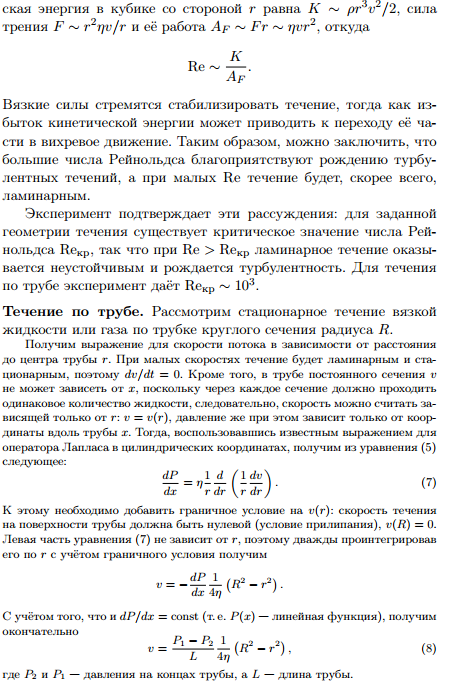
\includegraphics[width=16cm]{theory_4.png}
    	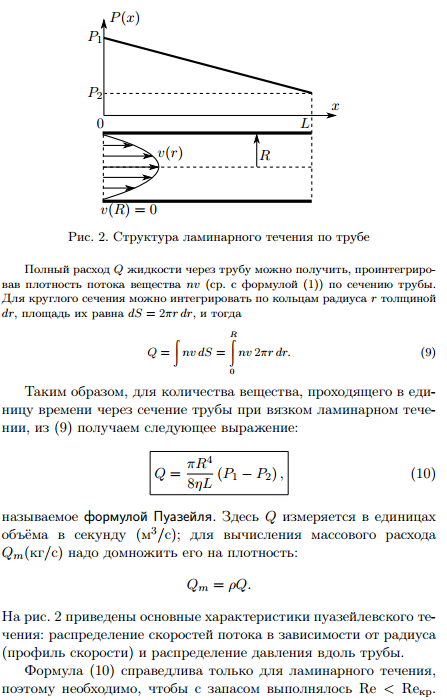
\includegraphics[width=16cm]{theory_5.png}
    	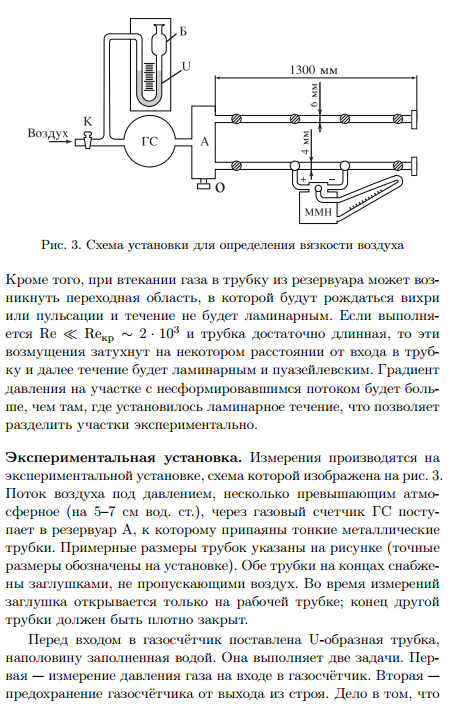
\includegraphics[width=16cm]{theory_6.png}
    	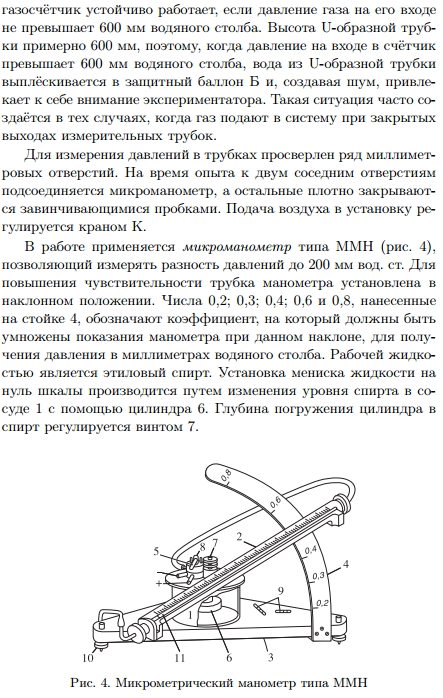
\includegraphics[width=16cm]{theory_7.png}
    	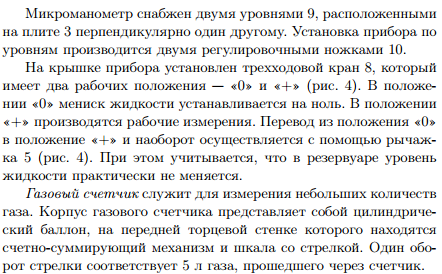
\includegraphics[width=16cm]{theory_8.png}
    \end{center}
    
    \begin{center}
    	\textbf{\large{Выполнение работы}}
    \end{center}
    
    Будем измерять вязкость воздуха, снимая зависимость разности давлений $\Delta P$ на некотором участке трубы от расхода воздуха $Q = \frac{\bigtriangleup V}{\bigtriangleup t}$, при этом $\bigtriangleup V$ измеряется газовым счетчиком, а $\bigtriangleup t$— секундомером. Измерения будем проводить на участках различной длины (50, 40 и 30 см) двух труб различных диаметров. Множитель на стойке микроманометра возьмём равным 0,2. Постепенно увеличим расход, начиная с маленьких перепадов давления.
    
    Будем вычислять $\eta$ из формулы Пуазейля(10).
    $\eta = \frac {\pi R ^ 4 \Delta P}{8 QL}$
    
    Оценку $Re$ получим из следующих соотношений: $Re = \frac{\rho vr}{\eta} = \frac{\rho lrS}{\eta tS} = \frac{\rho Q}{\eta \pi r}$
    
    При измерениях: $ \sigma_P = 1 $ деление (или 0.2 * 9.8 Па), $\sigma_{\Delta t} = 0.5c$
    \newline
    К сожалению, в некоторых сериях испытаний течение слишком быстро становится турбулентным, и коэффициент наклона приходится вычислять всего по двум-трём точкам из-за чего и погрешность выходит значительной.
    \newline
    
    Первая труба, $d=3,85 \pm 0.05 мм$
    
    1. $L = 50 cm$
    
    \begin{center}
    	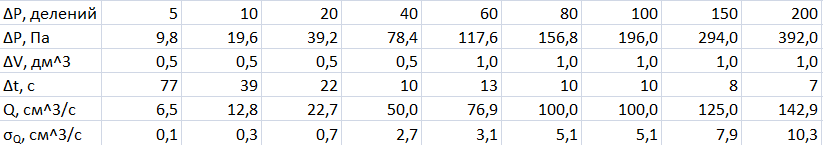
\includegraphics[width=10cm]{table1.png}
    	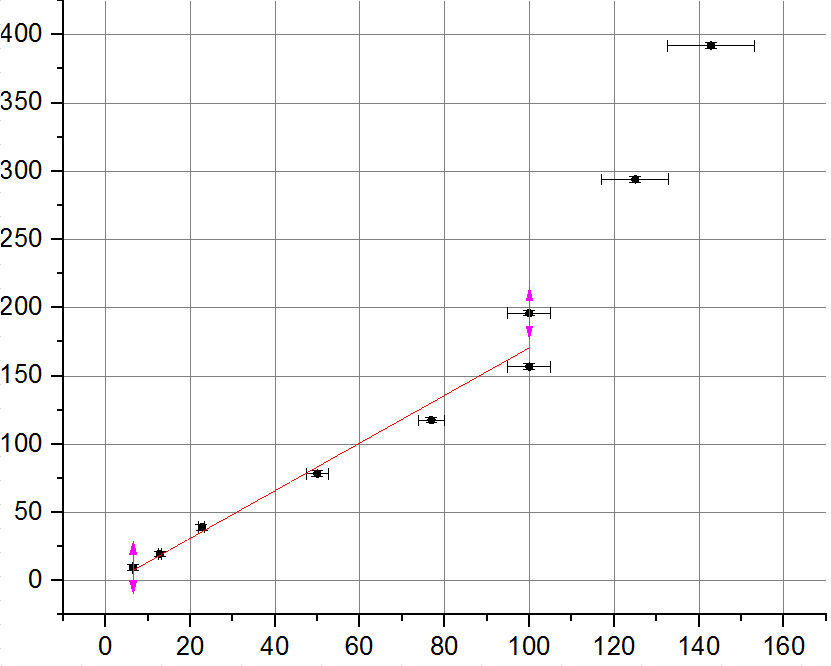
\includegraphics[width=10cm]{graph1.png}
    \end{center}
    
    Найденный тангенс угла наклона $k=(1,74 \pm 0,15) Па * с /см^3$. Теперь можно найти $\eta = (1,87 \pm 0,17) * 10^{-5} Па*с$ и $Re \approx 1223$
    
    2. $L = 40cm$
    
    \begin{center}
    	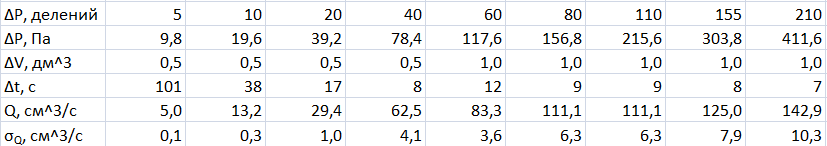
\includegraphics[width=10cm]{table2.png}
    	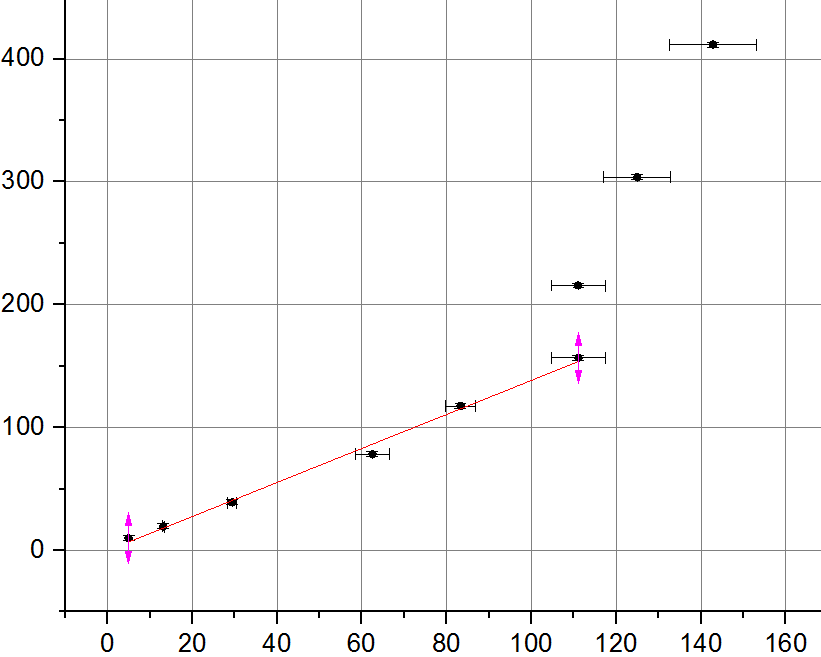
\includegraphics[width=10cm]{graph2.png}
    \end{center}
    
    Найденный тангенс угла наклона $k=(1,38 \pm 0,12) Па*с/см^3$
    
    $\eta = (1,86 \pm 0,17) * 10^{-5} Па*с$
    
    $Re \approx 1160$
    
    3. $L = 30cm$
    
    \begin{center}
    	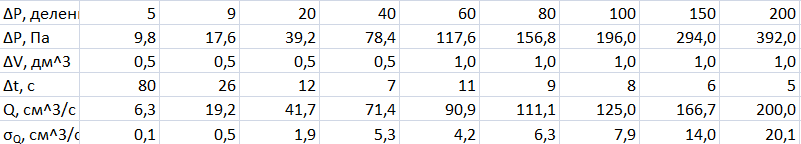
\includegraphics[width=10cm]{table3.png}
    	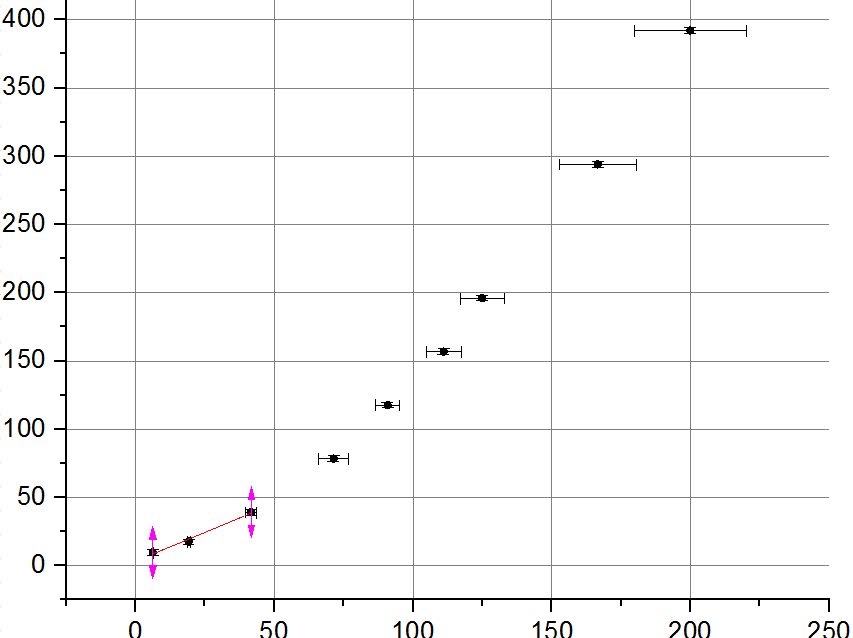
\includegraphics[width=10cm]{graph3.png}
    \end{center}
    
    Найденный тангенс угла наклона $k=(0,9 \pm 0,1) Па*с/см^3$
    
    $\eta = (1,61 \pm 0,15) * 10^{-5} Па*с$
    
    $Re \approx 963$
    
    Вторая труба, $d=5,85 \pm 0.05 мм$
    
    4. $L = 50cm$
    
    \begin{center}
    	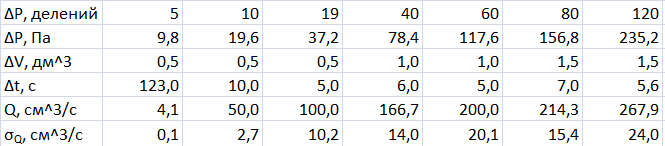
\includegraphics[width=10cm]{table4.png}
    	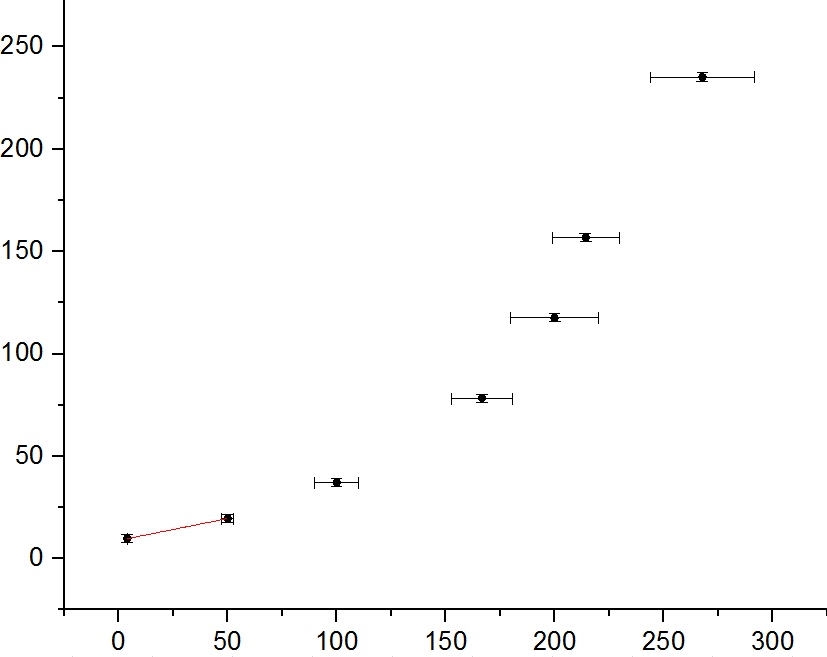
\includegraphics[width=10cm]{graph4.png}
    \end{center}
    
    Найденный тангенс угла наклона $k=(0,21 \pm 0,04) Па*с/см^3$
    
    $\eta = (1,2 \pm 0,3) * 10^{-5} Па*с$
    
    $Re \approx 1042$
    
    5. $L = 40cm$
    
    \begin{center}
    	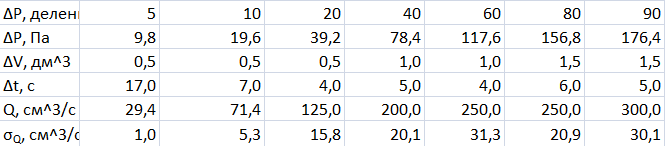
\includegraphics[width=10cm]{table5.png}
    	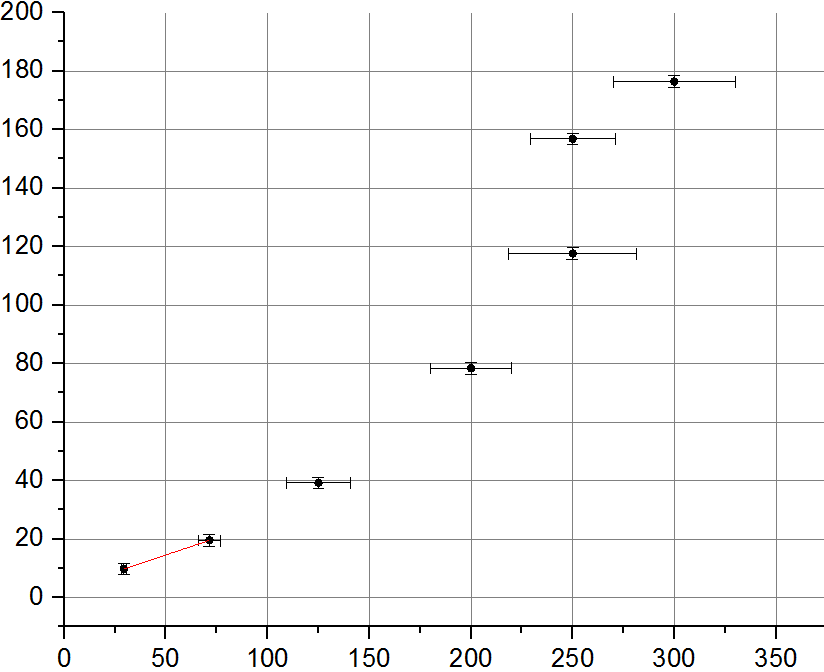
\includegraphics[width=10cm]{graph5.png}
    \end{center}
    
    Найденный тангенс угла наклона $k=(0,23 \pm 0,4) Па*с/см^3$
    
    $\eta = (1,6 \pm 0,3) * 10^{-5} Па*с$
    
    $Re \approx 916$
    
    6. $L = 30cm$
    
    \begin{center}
    	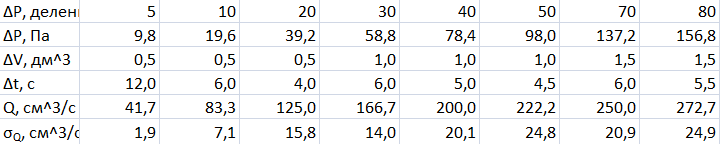
\includegraphics[width=10cm]{table6.png}
    	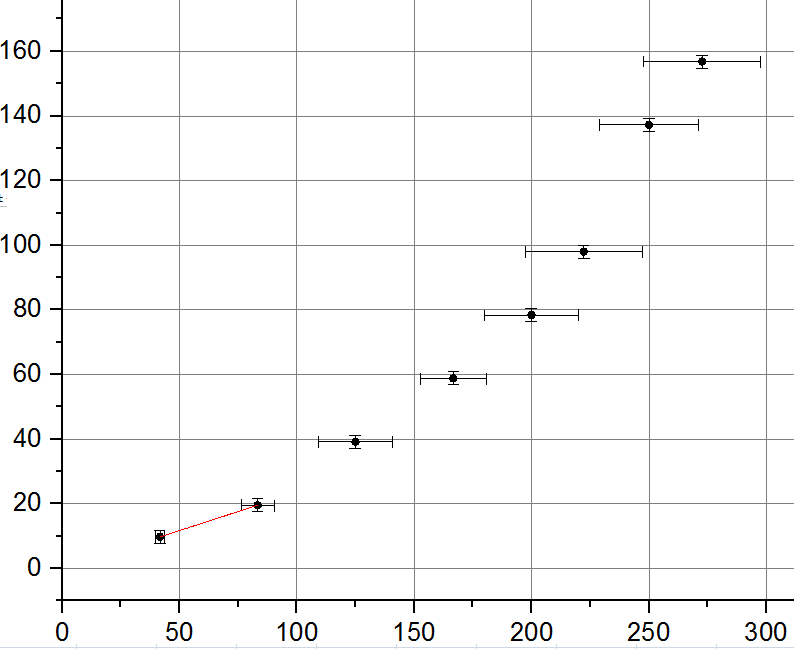
\includegraphics[width=10cm]{graph6.png}
    \end{center}
    
    Найденный тангенс угла наклона $k=(0,24 \pm 0,06) Па*с/см^3$
    
    $\eta = (2,3 \pm 0,5) * 10^{-5} Па*с$
    
    $Re \approx 751$
    \\ \\
    
    Сравним с теоретическими вычислениями. 
    
    Табличное значение вязкости при $T=300K$ $\eta = 18,5 * 10^{-6} Па*с$
    
    При $\lambda = 10^{-5} cm$, $T=293K$
    
    $\eta_{th} = \frac{1}{3} \rho v_T \lambda = \frac{1}{3} \rho \lambda \sqrt{\frac{3RT}{m_{mol}}} \approx  2,01 \cdot 10^{-5} Па*с$
    
    Как видим, в большинстве случаев, наши результаты в пределах погрешности подтверждают теоретические рассчёты.
    
\end{document}